\documentclass[tikz,border=5mm]{standalone}
\usepackage{tikz}
\usepackage{amsmath}
\usetikzlibrary{arrows.meta, positioning, calc}

\begin{document}

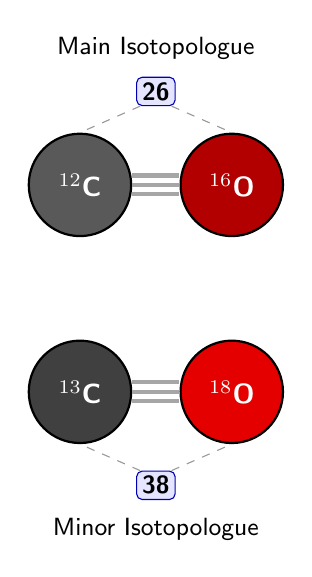
\begin{tikzpicture}
   [
      atom/.style={circle, draw, thick, minimum size=1.3cm, font=\sffamily\bfseries\color{white}},
      bond/.style={line width=1.5pt, gray!70},
      label node/.style={text=black, font=\sffamily\small},
      guide line/.style={thin, gray!80, dashed},
      number box/.style={rectangle, draw=blue!70!black, fill=blue!10,
                         rounded corners=2pt, inner sep=2pt,
                         font=\sffamily\bfseries\small}
   ]

   % =======================================================
   % Top Molecule: Main Isotopologue (12C, 16O) - 26
   % =======================================================

   % Atoms
   \node[atom, fill=gray!70!black] (C_top) {$^{12}\text{C}$};
   \node[atom, fill=red!70!black, right=0.6cm of C_top] (O_top) {$^{16}\text{O}$};

   % Triple bond (three parallel lines)
   \draw[bond] ($(C_top.east) + (0,0.12)$) -- ($(O_top.west) + (0,0.12)$);
   \draw[bond] (C_top) -- (O_top);
   \draw[bond] ($(C_top.east) - (0,0.12)$) -- ($(O_top.west) - (0,0.12)$);

   % Midpoint coordinate for centring labels
   \path let \p1 = (C_top), \p2 = (O_top) in
      coordinate (mid_top) at ($(\p1)!.5!(\p2)$);

   % Isotopologue Designation (26)
   \node[number box, above=1cm of mid_top] (num26) {26};

   % Guide lines from number box to both atoms
   \draw[guide line] ($(num26.south) - (0.2cm, 0)$) -- (C_top.north);
   \draw[guide line] ($(num26.south) + (0.2cm, 0)$) -- (O_top.north);

   % Label
   \node[label node, above=0.1cm of num26.north] {Main Isotopologue};

   % =======================================================
   % Bottom Molecule: Minor Isotopologue (13C, 18O) - 38
   % =======================================================

   % Atoms (below)
   \node[atom, fill=gray!50!black, below=1.3cm of C_top] (C_bottom) {$^{13}\text{C}$};
   \node[atom, fill=red!90!black, right=0.6cm of C_bottom] (O_bottom) {$^{18}\text{O}$};

   % Triple bond (three parallel lines)
   \draw[bond] ($(C_bottom.east) + (0,0.12)$) -- ($(O_bottom.west) + (0,0.12)$);
   \draw[bond] (C_bottom) -- (O_bottom);
   \draw[bond] ($(C_bottom.east) - (0,0.12)$) -- ($(O_bottom.west) - (0,0.12)$);

   % Midpoint coordinate for centring labels
   \path let \p3 = (C_bottom), \p4 = (O_bottom) in
      coordinate (mid_bottom) at ($(\p3)!.5!(\p4)$);

   % Isotopologue Designation (38)
   \node[number box, below=1cm of mid_bottom] (num38) {38};

   % Guide lines from number box to both atoms
   \draw[guide line] ($(num38.north) - (0.2cm, 0)$) -- (C_bottom.south);
   \draw[guide line] ($(num38.north) + (0.2cm, 0)$) -- (O_bottom.south);

   % Label
   \node[label node, below=0.1cm of num38.south] {Minor Isotopologue};

\end{tikzpicture}

\end{document}
